%% $Id: arbitrage.tex 13 2014-05-04 09:22:26Z natalie $
%% $HeadURL: https://server3.subversion-server.com/natp/svn/arbitrage/arbitrage.tex $
%% $Date: 2014-05-04 11:22:26 +0200 (Sun, 04 May 2014) $
%% $Revision: 13 $
%% $Author: natalie $

\documentclass[10pt,mathserif,notes=show]{beamer}
\newcounter{fulltoc}
\setbeamertemplate{blocks}[rounded][shadow=true]
\usepackage{sfmath}

%\documentclass[9pt,mathserif]{beamer}

% \documentclass[11pt,a4paper]{article}
% \usepackage{beamerarticle}
% \usepackage{fullpage}

%\usefonttheme{professionalfonts}
%\usepackage{sfmath} %% Makrele
\usepackage{graphicx,amsmath,amssymb,tikz,psfrag,bm}
\usepackage{booktabs} % professional tables
%\usepackage{dcolumn} % also supporting tables (alignment in stargazer function)
 \graphicspath{{_pics/}}

\usepackage{color}
%\usepackage{graphicx,color}
% Makrele helps to STRG+F through the PDF file and find all comments.
\providecommand{\cfw}[1]{\textcolor{magenta}{\textit{Makrele: }#1}}
\providecommand{\nat}[1]{\textcolor{red}{#1}}

% \usepackage[ngerman]{babel}
\usepackage{slashbox}
\renewcommand{\contentsname}{Overview} 
\usepackage{adjustbox}  % scaling function (e.g. scale tables to \textwidth)

%\usepackage{subcaption}  %% Makrele
\usepackage{hyperref}
\usepackage{graphics}
\usepackage{natbib}
\bibpunct{(}{)}{;}{a}{,}{,}
%\bibliographystyle{plainnat}

\usepackage[official,right]{eurosym}
\providecommand{\meur}[1]{\text{\EUR{#1}}} %%
\newcommand{\argmax}{\operatornamewithlimits{argmax}}
\newcommand{\argmin}{\operatornamewithlimits{argmin}}

\usepackage{setspace}
\setstretch{1.15}

\providecommand{\osigma}{\ensuremath{\overline\sigma}}
\providecommand{\vloan}{\ensuremath{V_{\text{loan}}}}
\providecommand{\vtranche}{\ensuremath{V}}
\providecommand{\bpvrei}{\ensuremath{\text{PV01}_{i,RE}}}
\providecommand{\bpvre}{\ensuremath{\text{PV01}_{RE}}}


%% formatting

\addtolength{\leftmargini}{-5pt}
\addtolength{\leftmargini}{-5pt}

\setbeamerfont*{itemize/enumerate subbody}{parent=itemize/enumerate body}
\setbeamerfont*{itemize/enumerate subsubbody}{parent=itemize/enumerate
  body}

\mode<presentation>
{
\usetheme{default}
}
\setbeamertemplate{navigation symbols}{}
\usecolortheme[rgb={0.13,0.28,0.59}]{structure}
\setbeamertemplate{itemize subitem}{--}
\setbeamertemplate{frametitle} {
	\begin{center}
	  {\large\bf \insertframetitle}
	\end{center}
}
      
\definecolor{structureBlue}{rgb}{0.13, 0.28, 0.59}
%\setbeamercolor{math text}{use=alerted text,fg=structure} %fsblue}
\setbeamercolor{math text}{use=alerted text,fg=structureBlue} %fsblue}
\setbeamerfont{alerted text}{series=\bfseries}
\setbeamercolor{alerted text}{fg=black}

\newcommand\footlineon{
  \setbeamertemplate{footline} {
    \begin{beamercolorbox}[ht=2.5ex,dp=1.125ex,leftskip=.8cm,rightskip=.6cm]{structure}
      \footnotesize \insertsection\hfill
      % \footnotesize \insertsubsectionnumber.~\insertsubsectionhead
      \hfill
      N.\ Packham
      \hfill
      % \insertsubsubsection
      % \hfill
      {\insertframenumber}
    \end{beamercolorbox}
    \vskip 0.45cm
  }
}

\newcommand\footlineoff{
  \setbeamertemplate{footline} {
    \begin{beamercolorbox}[ht=2.5ex,dp=1.125ex,leftskip=.8cm,rightskip=.6cm]{structure}
      \footnotesize\hfill
      {\insertframenumber}
    \end{beamercolorbox}
    \vskip 0.45cm
  }
}

\footlineon

\setbeamertemplate{subsection in
  toc}{% \inserttocsubsectionnumber.~
  \ \ \ \inserttocsubsection\\}

\setcounter{tocdepth}{4}
\AtBeginSection[]
{
%  \begin{frame}[shrink]
%  \begin{frame}[squeeze]
\footlineoff
  \begin{frame}<beamer>
    \frametitle{Overview}
    \ifnum\value{fulltoc}<1
    \tableofcontents
    \addtocounter{fulltoc}{1}
    \else
    \tableofcontents[currentsubsection,hideothersubsections]
    \fi
  \end{frame}
  \footlineon
}

\AtBeginSubsection[]
{
\footlineoff
  \begin{frame}<beamer>
    \frametitle{Overview}
    \tableofcontents[currentsubsection,hideothersubsections,subsectionstyle=show/shaded/hide]
  \end{frame}
  \footlineon
}

\AtBeginSubsubsection[]
{
\footlineoff
  \begin{frame}<beamer>
    \frametitle{Overview}
    \tableofcontents[currentsubsection,hideothersubsections,subsectionstyle=show/shaded/hide]
  \end{frame}
  \footlineon
}

\providecommand{\structure}[1]{\usebeamercolor[fg]{structure}{#1}}
\setbeamerfont{block title}{size=\normalsize,series=\bfseries,parent=structure}


%% begin presentation
\title{\bigskip\bigskip\bigskip\\
  \bfseries{Copula-based hedging of cryptocurrencies}}


% \author{Prof.\ Dr.\ Natalie
%   Packham\\[3ex]
% Hochschule f\"ur Wirtschaft und Recht Berlin}
\author{{\bf Natalie Packham\medskip\\} joint work with\\ Francis Liu,
  Meng-Jou Lu, Wolfgang K.\ H\"ardle}
\date{
  \vspace*{-1.5\baselineskip}

  Mathfinance Conference\\
  16 March 2021\\

\hspace*{-.75cm}
  
\includegraphics[width=4cm]{HWR_Logo_RGB.pdf}
  \hspace*{1cm}
  % 
\includegraphics[width=2cm]{_pics/IRTG.pdf}
  \hspace*{2cm}
  \hspace*{2.25cm}
    
\includegraphics[width=2cm]{HU.png}
}
\logo{
}
%

%\setbeameroption{show notes}

\renewcommand{\(}{\begin{columns}}
\renewcommand{\)}{\end{columns}}
\newcommand{\<}[1]{\begin{column}{#1}}
\renewcommand{\>}{\end{column}}
%%%%%%%%%%%%%%%%%%%%%%%%%%%%%%%%%%%%%%%%%%%%%%%%%%

\newtheorem{proposition}[theorem]{Proposition}
\newtheorem*{remark}{Remark}

\theoremstyle{definition}
\newtheorem{condition}{Condition}
\newtheorem*{iproof}{Proof}
\newtheorem{algorithm}{Algorithm}
\newtheorem{assumption}{Assumption}

\providecommand{\I}{\text{i}}
\newcommand{\CFS}{\mathfrak{B}} %functions with Fourier transform having compact support.
\DeclareMathOperator{\C}{C}
\providecommand{\CFCS}{C_c(\R)} %continuous functions with compact support.
\providecommand{\Pb}{\mathbb P}
\providecommand{\IF}{\mathbf{1}}
\newcommand{\Four}[1]{\mathfrak{F}(#1)} %Fourier transform
\newcommand{\FourInv}[1]{\mathfrak{F}^{(-1)}\left(#1\right)} %Fourier inversion
\providecommand{\call}{\gamma} %modified call price
\providecommand{\tg}{\tilde{g}}
\providecommand{\tp}{\tilde{p}}
%%
%% $Id: Definitions.tex,v 1.6 2008/07/26 14:55:50 natalie Exp $
%% $Source: /Users/natalie/cvs/tex/dynamics/Definitions.tex,v $
%% $Date: 2008/07/26 14:55:50 $
%% $Revision: 1.6 $
%%

%\usepackage{mathrsfs}

%% GENERAL DEFINITIONS
\unitlength1cm

%% COMMAND DEFINITIONS
\newcommand{\E}{{\mathbb{E}}}
%%\renewcommand{\E}{{\mathds E}}
%%\renewcommand{\E}{{\varmathbb{E}}}
%%\renewcommand{\E}{{\mathrm{I\!E}}}
\providecommand{\R}{{\mathbb{R}}}
\newcommand{\T}{{\mathbb{T}}}
\newcommand{\Fb}{{\mathbb{F}}}
\newcommand{\Eqn}{{\mathbb{E}}_{{\bf Q}_N}}
\newcommand{\Eq}{{\mathbb{E}}_{{\bf Q}}}
\newcommand{\Eqm}{{\mathbb{E}}_{{\bf Q}_M}}
\newcommand{\EqT}{{\mathbb{E}}_{{\bf Q}_T}}
\newcommand{\EqTz}{{\mathbb{E}}_{{\bf Q}_{T_2}}}
\newcommand{\EqTe}{{\mathbb{E}}_{{\bf Q}_{T_1}}}
\newcommand{\EqSe}{{\mathbb{E}}_{{\bf Q}_{S^1}}}
\newcommand{\EqSz}{{\mathbb{E}}_{{\bf Q}_{S^2}}}
\newcommand{\p}{{\bf P}}
%%\renewcommand{\p}{{\mathds{P}}}
%%\renewcommand{\p}{{\varmathbb{P}}}
%%\renewcommand{\p}{{\mathrm{I\!P}}}
\newcommand{\pas}{\text{{\bf P}--a.s.}}
\newcommand{\paa}{\text{{\bf P}--a.a.}}
\newcommand{\qas}{\text{{\bf Q}--a.s.}}
\newcommand{\e}{{\bf e}}
\newcommand{\q}{{\bf Q}}
\newcommand{\qn}{{\bf Q}_N}
\newcommand{\qm}{{\bf Q}_M}
\newcommand{\qT}{{\bf Q}_T}
\newcommand{\qTz}{{\bf Q}_{T_2}}
\newcommand{\qTe}{{\bf Q}_{T_1}}
\newcommand{\qS}{{\bf Q}_S}
\newcommand{\qSe}{{\bf Q}_{S^1}}
\newcommand{\qSz}{{\bf Q}_{S^2}}
\newcommand{\F}{{\cal F}}
\newcommand{\G}{{\cal G}}
\newcommand{\A}{{\cal A}}
\newcommand{\Hc}{{\cal H}}
\newcommand{\dP}{{\rm d}{\bf P}}
\newcommand{\du}{{\rm d}u}
%%\newcommand{\dt}{{\rm d}t}
\newcommand{\dd}{{\rm d}}
\newcommand{\df}{{\rm \bf DF}}
\providecommand{\N}{{\mathbb N}}
\providecommand{\Ncdf}{{\rm N}}
%\renewcommand{\Ncdf}{{\Phi}}
\newcommand{\n}{{\rm n}}
\newcommand{\emb}{\bf \em}
\newcommand{\1}{\textbf{1}}
\newcommand{\qs}{{\q_{\rm Swap}}}
\newcommand{\fx}{{\rm fx}}
\newcommand{\V}{{\rm Var}}
%\newcommand{\C}{{\bf C}}
\newcommand{\Om}{{\Omega}}
\providecommand{\limn}{\ensuremath{\lim_{n\rightarrow\infty}}}
\providecommand{\qv}[2]{\ensuremath{\langle #1,#1\rangle_{#2}}}

%% ENVIRONMENT DEFINITIONS
%\newtheorem{prop}{Proposition}[section]
%\newtheorem{theo}{Theorem}[section]
%\newtheorem{lem}{Lemma}[section]
%\newtheorem{ass}{Assumption}[section]
%\newtheorem{cor}{Corollary}[section]
%\newtheorem{aufg}{Exercise}[section]
%\newtheorem{defi}{Definition}[section]

\ifx\prop\undefined
\newtheorem{prop}{Proposition}[section]
\fi
\newtheorem{theo}[prop]{Theorem}
\newtheorem{lem}[prop]{Lemma}
\newtheorem{cor}[prop]{Corollary}
\newtheorem{defi}[prop]{Definition}

%% enumeration in lists
\providecommand{\labelenumi}{{\rm (\roman{enumi})}}
   %\setlength{\topsep}{0cm}
    \setlength{\labelsep}{0.3cm}
    %\setlength{\itemindent}{0cm}
   \setlength{\leftmargin}{10cm}
    \setlength{\labelwidth}{5cm}

\providecommand{\cadlag}{c\`adl\`ag }
\providecommand{\cadlagns}{c\`adl\`ag}
\providecommand{\caglad}{c\`agl\`ad }
\providecommand{\cad}{c\`ad}
\providecommand{\cag}{c\`ag}
\providecommand{\levy}{L\'evy\ }
\providecommand{\levyns}{L\'evy}
\providecommand{\levyito}{L\'evy-It\^o\ } 
\providecommand{\levykhinchin}{L\'evy-Khinchin\ }
\providecommand{\D}{\ensuremath{D(\R_+,\R)}}
\providecommand{\Dsig}{\ensuremath{D(\R_+, \R_+\setminus\{0\}})}
\providecommand{\Dd}{\ensuremath{D(\R_+,\R^d)}}
\providecommand{\C}{\ensuremath{C(\R_+,\R)}}
\providecommand{\Cd}{\ensuremath{C(\R_+,\R^d)}}
\providecommand{\rpos}{\ensuremath{{[0,\infty)}}}

\def\Z{{\mathbb Z}}
%\def\N{{\mathbb N}}
%\def\R{{\mathbb R}}
%\def\C{{\mathbb C}}
%\def\H{{\mathbb H}}
\def\P{{\mathbb P}}
\def\Q{{\mathbb Q}}
%\def\E{{\mathbb E}}
\def\I{{\mathbb I}}
%\def\T{{\mathbb T}}
%\def\F{{\mathbb F}}
\def\M{{\mathbb M}}
%\def\Hc{{\mathcal H}}
\def\Mc{{\mathcal M}}
\def\filtration#1{{\ensuremath\mathcal{#1}}}
%\def\filt{{\mathcal F}}
\def\tp{\tilde{\p}}
\providecommand{\vec}[1]{\ensuremath{\bm #1}}
\providecommand{\vecb}[1]{\ensuremath{\bm #1}}
\providecommand{\abs}[1]{\ensuremath{\lvert#1\rvert}}
\providecommand{\norm}[1]{\ensuremath{\lVert#1\rVert}}
\providecommand{\var}{\ensuremath{\text{Var}}}
\providecommand{\cov}{\ensuremath{\text{Cov}}}
\providecommand{\borel}[0]{\ensuremath{\mathcal{B}}}
\providecommand{\intinf}[0]{\ensuremath{\int_{-\infty}^\infty}}
\providecommand{\intpos}[0]{\ensuremath{\int_0^\infty}}
\providecommand{\intneg}[0]{\ensuremath{\int_{-\infty}^0}}
\providecommand{\todo}[1]{\footnote{#1}}
\providecommand{\dynkin}[0]{\ensuremath{\mathcal D}}
\providecommand{\ce}[2]{\ensuremath{\E(#1|\filtration{#2})}}
\providecommand{\inv}[1]{\ensuremath{#1^{(-1)}}}
\providecommand{\os}[2]{\ensuremath{#1^{(#2)}}}
\providecommand{\pos}[2]{\ensuremath{h_{#1}(#2)}}
%\providecommand{\poslong}[2]{\ensuremath{h(#1, #2)}}
\providecommand{\poslong}[3]{\ensuremath{h_{#1, #2}(#3)}}

%% Class of finite variation processes
\providecommand{\classfv}{\ensuremath{\mathscr V}}
\providecommand{\classv}{\ensuremath{\mathscr V}}
%% Stochastic integral operator
\providecommand{\stint}{\ensuremath{\cdotp}}
\providecommand{\classh}{\ensuremath{\mathscr H^2}}
\providecommand{\classhloc}{\ensuremath{\mathscr H^2_{\rm loc}}}
\providecommand{\classm}{\ensuremath{\mathscr M}}
\providecommand{\classmloc}{\ensuremath{\mathscr M_{\rm loc}}}
\providecommand{\classl}{\ensuremath{L^2}}
\providecommand{\classlloc}{\ensuremath{L^2_{\rm loc}}}
\providecommand{\classa}{\ensuremath{\mathscr A}}
\providecommand{\classaloc}{\ensuremath{\mathscr A_{\rm loc}}}
\providecommand{\classalocpos}{\ensuremath{\mathscr A_{\rm loc}^+}}
\providecommand{\classp}{\ensuremath{\mathscr P}}
\providecommand{\classo}{\ensuremath{\mathscr O}}
\providecommand{\classs}{\ensuremath{\mathscr S}}
\providecommand{\classsp}{\ensuremath{\mathscr S_p}}
\providecommand{\nullset}{\ensuremath{\mathscr N}}

\providecommand{\ito}{It\^o }
\providecommand{\itos}{It\^o's\, }

\providecommand{\variation}[2]{\ensuremath{\rm V_{#1}(#2)}}
\renewcommand{\H}{\ensuremath{\mathcal H}}
%% CPO distribution
\providecommand{\cpo}{\ensuremath{{\rm CPO}}}
\providecommand{\Fsigma}{\ensuremath{\mathcal \F_\infty^\sigma}}
\providecommand{\sigd}{\ensuremath{\mathscr D}}

%% Credit spreads
\providecommand{\s}{{\bf s}}
\providecommand{\classu}{\ensuremath{\mathscr U}}

\providecommand{\sX}{\ensuremath{\mathcal X}}
\providecommand{\sY}{\ensuremath{\mathcal Y}}
\providecommand{\dx}{\ensuremath{\frac{\partial}{\partial x}}} %%
\providecommand{\dt}{\ensuremath{\frac{\partial}{\partial t}}} %%
\providecommand{\dy}{\ensuremath{\frac{\partial}{\partial y}}} %%
\newcommand{\argmax}{\operatornamewithlimits{argmax}}
\newcommand{\argmin}{\operatornamewithlimits{argmin}}



\begin{document}

\frame{ \thispagestyle{empty} \titlepage }

\logo{}

%%%%%%%%%%%%%%%%%%%%%%%%%%%%%%%%%%%%%%%%%%%%%%%%%%%%%%
%%%%%%%%%%%%%%%%%%%%%%%%%%%%%%%%%%%%%%%%%%%%%%%%%%%%%%
% \begin{frame}{Introduction}
%   \tableofcontents
% \end{frame}

%%%%%%%%%%%%%%%%%%%%%%%%%%%%%%%%%%%%%%%%%%%%%%%%%%%%%%
%%%%%%%%%%%%%%%%%%%%%%%%%%%%%%%%%%%%%%%%%%%%%%%%%%%%%%


\setcounter{tocdepth}{2}%


\section{Motivation}

\begin{frame}
  \frametitle{Digital assets are here to stay}
  \begin{itemize}
      \addtolength{\itemsep}{3pt}
  \item Markets for cryptocurrencies are maturing:
    \begin{itemize}
      \addtolength{\itemsep}{3pt}
      \item Institutional investors are buying into it. 
      \item Regulators are working hard to make stablecoins “safe”
        (e.g.\ resolve issues of jurisdiction, financial stability).
      \item Exchanges (e.g.\ CME) are issuing futures and options. 
      \end{itemize}
    \end{itemize}
    \vspace*{.5\baselineskip}
    
  $\Longrightarrow$ We are in the middle of the digitalisation
  of financial markets...
  \\
  \pause
  \hfill (... and it's progressing rapidly.)
  % \item Hedging with futures
  % \item Literature
\end{frame}

\begin{frame}
  \frametitle{Digital assets are here to stay}
  \begin{center}
    
\includegraphics[scale=.25]{../_pics/ScreenshotGARP.pdf}
  \end{center}
  {\tiny \url{https://www.garp.org/\#!/risk-intelligence/market/investment-management/a1Z1W000005kZDGUA2}}
\end{frame}

\begin{frame}
  \frametitle{Bitcoin futures}
  \begin{itemize}
    \addtolength{\itemsep}{3pt}
  \item CME launched Bitcoin Futures in December 2017 and options on
    futures in January 2020
  \item Bitcoin Future:
    \begin{itemize}
    \item Underlying: Bitcoin Reference Rate (BRR), based on relevant
      bitcoin transaction onn certain exchanges
    \item Maturities: nearest two Decembers and nearest six consecutive
      months 
      \item Settlement: cash
    \end{itemize}
    \item {\footnotesize \url{https://www.cmegroup.com/trading/equity-index/us-index/bitcoin.html}}
  \end{itemize}
\end{frame}

\begin{frame}
  \frametitle{Hedging cryptos}
  \begin{itemize}
  \item Hedging Bitcoin exposure with Bitcoin futures: 
    \begin{itemize}
    \item Basis risk
    \item BRR not traded
    \item Ability of futures to hedge tail risks?
    \end{itemize}
    \pause
    \begin{minipage}[t]{.525\linewidth}
    \item Hedge other cryptos with Bitcoin?
      \begin{itemize}
      \item High correlation
      \item Tail risks, extreme events?
      \end{itemize}
    \end{minipage}
    \begin{minipage}[t]{.45\linewidth}
      \begin{center}
        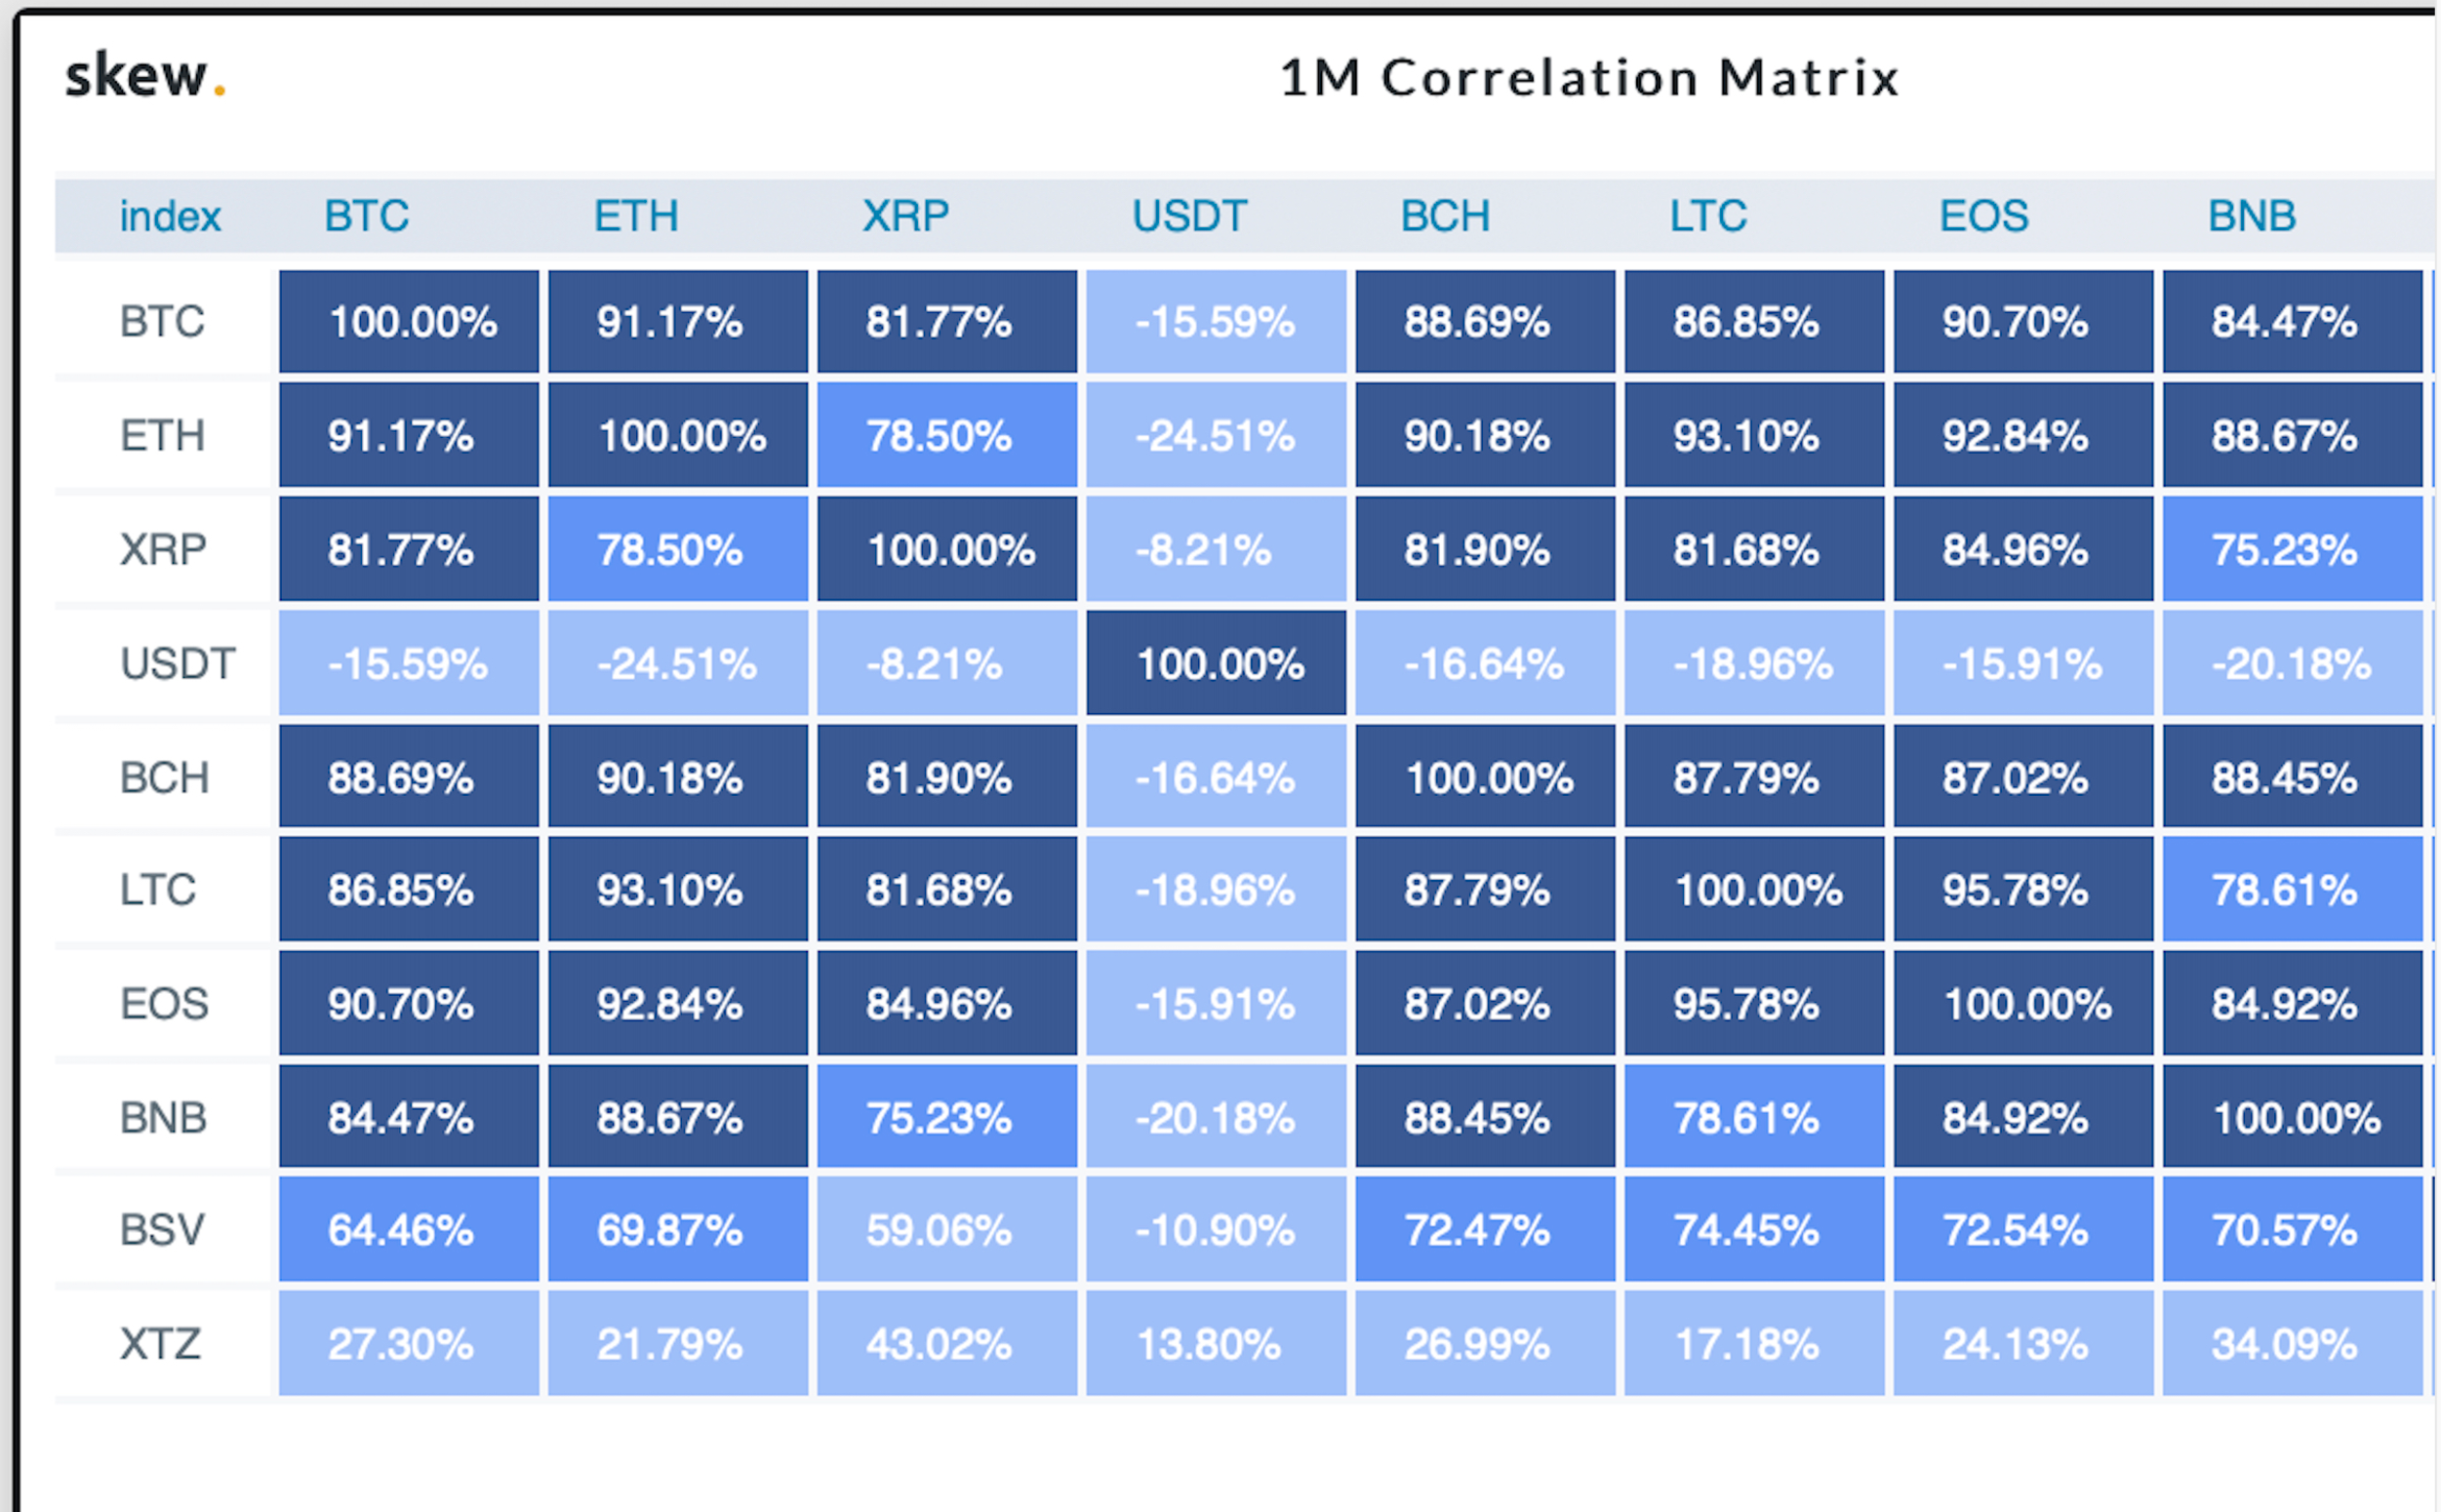
\includegraphics[scale=.125]{../_pics/SkewCorrelation.pdf}\\
        \hfill{\tiny Source: skew.com, December 2019}
      \end{center}
    \end{minipage}
    \vspace*{-4\baselineskip}
    \pause
    \item Two directions:
      \begin{itemize}
      \item Copulas
      \item Risk measures
      \end{itemize}
  \end{itemize}
\end{frame}


\section{Copula-based hedging}

\begin{frame}
  \frametitle{Hedging spot with futures}
  \begin{itemize}
      \addtolength{\itemsep}{3pt}
  \item Hedge portfolio return: $R_t^h = R_t^S - h\, R_t^F$, where
    \begin{itemize}
      \addtolength{\itemsep}{3pt}
    \item $R_t^S$: spot return at time $t$
    \item $R_t^F$: futures return at time $t$
    \item $h$: hedge ratio
    \end{itemize}
  \item Goal: Find optimal hedge ratio $h^\star$
  \item Minimum-variance hedge ratio, e.g. \cite{Ederington1979},
    assumes variance as risk measure and elliptical return
    distribution 
  \item Extensions: risk measures, copulas, e.g.\
    \citep{Harris2006,Barbi2014} 
  \end{itemize}
\end{frame}

\begin{frame}
  \frametitle{Copulas}
  \begin{definition}
    A (bivariate) {\bf copula} is a distribution function on $[0,1]^2$
    with standard uniform marginals.
  \end{definition}
  \begin{itemize}
  \item Copulas differ only through the dependence between the
    marginals.
  \item Sklar's Theorem (below) captures that copulas allow to
    separate
    \begin{itemize}
    \item modelling of the marginals, and
    \item modelling of the dependence structure.
    \end{itemize}
  \end{itemize}
\end{frame}

\begin{frame}
  \frametitle{Copulas}
  \begin{theorem}[Sklar's Theorem]
  Let $F$ be a joint distribution function with margins $F_1,
  F_2$. Then, there exists a copula $C:[0,1]^2\rightarrow[0,1]$ such
  that, for all $x,y\in \R$
  \begin{equation}
    \label{eq:4}
    F(x,y)=C(F_1(x), F_2(y)). 
  \end{equation}
  If the margins are continuous, then $C$ is unique; otherwise $C$ is
  unique on the range of the margins.

  Conversely, if $C$ is a copula and $F_1, F_2$ are univariate
  distribution functions, then the function $F$ defined by (\ref{eq:4})
  is a joint distribution function with margins $F_1, F_2$.
\end{theorem}
\begin{itemize}
  \addtolength{\itemsep}{1pt}
\item Representation of $C$ in terms of $F$ and its
  margins: 
  \begin{equation*}
    C(u,v) = F(F_1^{(-1)}(u), F_2^{(-1)}(v)). 
  \end{equation*}
  \vspace*{-1.1\baselineskip}
\end{itemize}
\end{frame}

\begin{frame}
  \frametitle{Examples of copulas}
  \begin{itemize}
  \item Gaussian, Student $t$, NIG factor, Gumbel, Clayton, Frank,
    Plackett, Gaussian Mixture
  \item Add scatterplots here
  \end{itemize}
\end{frame}


\begin{frame}
  \frametitle{Copula-based hedging}
  \begin{proposition}[\cite{Barbi2014}]
  \label{prop:dfrh}
  Let $R^S$ and $R^F$ be two real-valued random variables with
  corresponding 
  absolutely continuous copula $C_{R^S, R^F}$ and
  continuous marginals $F_{R^S}$ and $F_{R^F}$. Then, the distribution
  of of $R^h$ is given by
  \begin{equation}
    \label{eq:3}
    F_{R^h}(x) = 1- \int^1_0 D_1 C_{R^S, R^F}
    \left\{ u, F_{R^F} \left\{ \frac{F^{-1}_{R^S}(u)-x}{h} \right\}
    \right\}\, \dd u.
  \end{equation}
\end{proposition}
\begin{itemize}
\item Easy to show (e.g.\ \citet{McNeil2005}):
\begin{equation*}
  D_1 C_{X,Y}(F_X(x), F_Y(y)) = \frac{\partial}{\partial u} C(u,v) = \p(Y\leq y|X=x).
\end{equation*}
\end{itemize}
\end{frame}

\begin{frame}
  \frametitle{Risk measures}
  \begin{itemize}
    \addtolength{\itemsep}{5pt}
  \item {\bf Variance}: $\text{Var}(R^h)$
  \item {\bf Value-at-risk (VaR)}: $\text{VaR}_\alpha = -
    F_{R^h}^{(-1)}(1-\alpha)$  
  \item {\bf Expected Shortfall (ES)}: 
    $\displaystyle \text{ES}_\alpha =-
    \frac{1}{1-\alpha}\int_{-\infty}^{\alpha} F_{R^h}^{(-1)}(p) \dd p$.
  \end{itemize}
\end{frame}

\begin{frame}
  \frametitle{Risk measures}
  \begin{itemize}
    \addtolength{\itemsep}{3pt}
\item {\bf Spectral risk measures (SRM)} \citep{Acerbi2002,Cotter2006}:
    \begin{equation*}
      \rho_\phi = -\int_0^1 \phi(p)\, F_{R^h}^{(-1)}\, \dd p,
    \end{equation*}
    where $q_p$ is the $p$-quantile of the return distribution and
    $\phi(s)$, $s\in [0,1]$, is the so-called {\bf risk aversion
      function\/}, a weighting function such that 

    \hspace*{2cm}\begin{minipage}[t]{.7\linewidth}
      \vspace*{-.75\baselineskip}
      \begin{enumerate}[(i)]
        \addtolength{\itemsep}{3pt}
      \item $\phi(p)\geq 0$,
      \item $\int_0^1\phi(p)\, \dd p=1$,
      \item $\phi'(p)\leq 0$.
      \end{enumerate}
    \end{minipage}
  \item SRM's are coherent risk measures.
  \end{itemize}
\end{frame}

\begin{frame}
  \frametitle{Risk measures}
  \begin{itemize}
    \addtolength{\itemsep}{3pt}
  \item {\bf Exponential spectral risk measure}:
    weighting function $\phi(p) = \lambda \e^{-k(1-p)}$, where
    $\lambda$ is an unknown positive constant, derived from exponential
  utility function: 
  \begin{equation*}
    \rho_{\phi} = \int_0^1 \phi(p)\, F^{(-1)}(p)\, \dd p =
    \frac{k}{1-\e^{-k}} \int_0^1 \e^{-k(1-p)}\, F^{(-1)}(p)\, \dd p. 
  \end{equation*}
\end{itemize}
\end{frame}

\begin{frame}
  \frametitle{Optimal hedge ratio}
  \begin{itemize}
    \addtolength{\itemsep}{3pt}
  \item Hedge portfolio: $R_t^h = R_t^S - h R_t^F$, with $h$ hedge
    ratio
  \item Optimal hedge ratio:
    \begin{equation*}
h^\ast = \argmin_h \rho(h),% _\phi(s,h),
\end{equation*}
where $\rho(h)$ is the risk of the hedge portfolio with hedge ratio
$h$. 
%  for given
% confidence level $1-s$ (if applicable, e.g.\ in the case of VaR, ES),
% where $\rho_\phi$ is a spectral risk measure with weighting function
% $\phi$ (see below).
  \end{itemize}
\end{frame}

\section{Data}

\begin{frame}
  \frametitle{Data}
  \begin{itemize}
  \item Daily log returns, 23pm CET
  \item 29 May 2018 through 3 Feb 2021
  \item Spot: Coingecko Bitcoin / USDC 
  \item Future: CME BTC Future
  \end{itemize}
\end{frame}

\begin{frame}
  \frametitle{Summary statistics}
  {\small%
\begin{center}

\begin{tabular}{lr@{.}lr@{.}lr@{.}lr@{.}l}
Variable & \multicolumn{2}{c}{Mean}
 & \multicolumn{2}{c}{Median}
  & \multicolumn{2}{c}{Minimum}
   & \multicolumn{2}{c}{Maximum} \\[1ex]
BTC spot& 0&0023782 & 0&0013855 & $-$0&28846 & 0&23522\\
Future & 0&0023970 & 0&0012540 & $-$0&26773 & 0&22251\\[10pt]

Variable &  \multicolumn{2}{c}{Std.\ Dev.}
 & \multicolumn{2}{c}{C.V.}
  & \multicolumn{2}{c}{Skewness}
   & \multicolumn{2}{c}{Ex.\ kurtosis} \\[1ex]
BTC spot & 0&043133 & 18&137 & $-$0&27245 & 5&8658\\
Future & 0&046288 & 19&311 & $-$0&27321 & 5&4709\\[10pt]

Variable &  \multicolumn{2}{c}{5\% perc.}
 & \multicolumn{2}{c}{95\% perc.}
  & \multicolumn{2}{c}{IQ Range}
   & \multicolumn{2}{c}{Missing obs.} \\[1ex]
BTC spot & $-$0&065328 & 0&072665 & 0&033819 & \multicolumn{2}{c}{0}\\
Future & $-$0&066085 & 0&077146 & 0&037142 & \multicolumn{2}{c}{0}\\
\end{tabular}
\end{center}
}
\end{frame}

\begin{frame}
  \frametitle{Time series}
  \begin{center}
    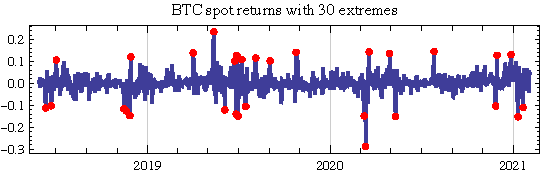
\includegraphics[scale=1]{../_pics/btc_series.pdf}\\
    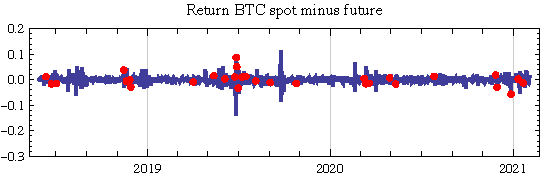
\includegraphics[scale=1]{../_pics/btc_vs_future_series.pdf}    
  \end{center}
\end{frame}

\begin{frame}
  \frametitle{Distribution}
  \begin{center}
    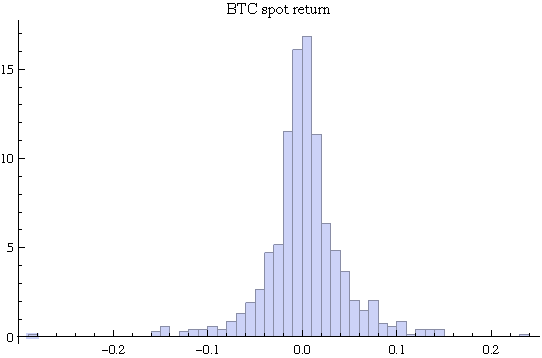
\includegraphics[scale=1]{../_pics/btc_hist.pdf}
  \end{center}
  \begin{itemize}
  \item Student $t$ distribution: $\nu=7.95$
  \item Tail / Generalised Pareto distribution: tail index $1/\xi=4.92$ 
  \end{itemize}
\end{frame}

\begin{frame}
  \frametitle{QQ-plot}
  \begin{center}
    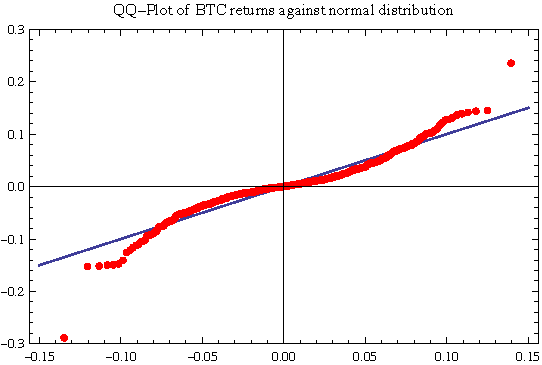
\includegraphics[scale=1]{../_pics/btc_qq.pdf}
  \end{center}
\end{frame}

\begin{frame}
  \frametitle{Spot and Future}
  \begin{center}
    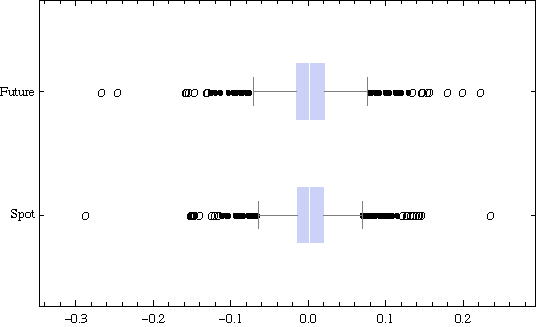
\includegraphics[scale=1]{../_pics/btc_future_box.pdf}
  \end{center}
\end{frame}

\begin{frame}
  \frametitle{Spot and Future}
  \begin{center}
    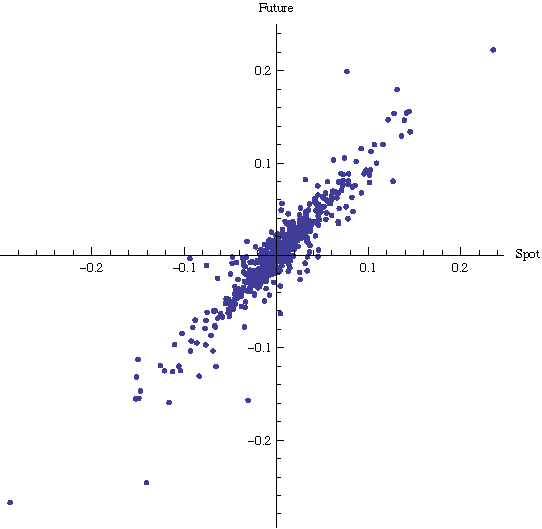
\includegraphics[scale=1]{../_pics/btc_future_scatter.pdf}
  \end{center}
\end{frame}

\section{Results}

\begin{frame}
  \frametitle{Hedge Effectiveness}
  \begin{itemize}
  \item Hedge effectiveness \citep{Ederington1979} captures percentage
    reduction in risk:
    \begin{equation*}
      1- \frac{\rho(R^h)}{\rho(R^S)}.
    \end{equation*}
  \item Optimisation of $h^\ast$ every 30 days based on
    300-day-window. 
  \end{itemize}
\end{frame}

\begin{frame}
  \frametitle{Hedge effectiveness}
  
\end{frame}

\begin{frame}
  \frametitle{P\&L}
  
\end{frame}

\begin{frame}
  \frametitle{Optimal hedge parameters}
  \end{frame}

\section*{}

\bibliographystyle{abbrvnamed}
%\bibliographystyle{plainnat}%
\begin{frame}[allowframebreaks]
  \frametitle{References} {\footnotesize %
    \bibliography{finance} %
  }
\end{frame}


\footlineoff

\section*{}

\begin{frame}
 \begin{center}
   \vspace{3.5cm}
   \large{\bf Thank you!}
   % \vspace{1cm}
 \end{center}
 \vspace{.5cm}
  \begin{columns}[b]
    \column{.5\linewidth} \scalebox{.75}{ %
      \begin{minipage}{1.2\linewidth}
        {\bf Prof.\ Dr.\ Natalie Packham}\\
        Professor of Mathematics and Statistics\\
        Berlin School of Economics and Law\\
	Badensche Str.\ 52\\
        10825 Berlin\\
        \href{mailto:natalie.packham@hwr-berlin.de}{natalie.packham@hwr-berlin.de}
      \end{minipage}
    } %
    \vspace{0pt} \column{.5\linewidth}

    \hfill
\includegraphics[width=2cm]{IRTG.pdf}
    \vspace*{\baselineskip}

    \hfill
\includegraphics[width=3cm]{HWR_Logo_RGB.pdf}
    
\includegraphics[width=2cm]{HU.png}
    \vspace{0pt}
  \end{columns}
  \vspace{.5cm}
\end{frame}

\end{document}



